% !TeX encoding = UTF-8
% !TeX spellcheck = en_US

\section{Introduction}

\subsection{Running Example}
	\begin{frame}
		\frametitle{Introduction}
		\framesubtitle{Running Example: She Remembered Caterpillars}
		\begin{center}
			\vspace{-4mm}
			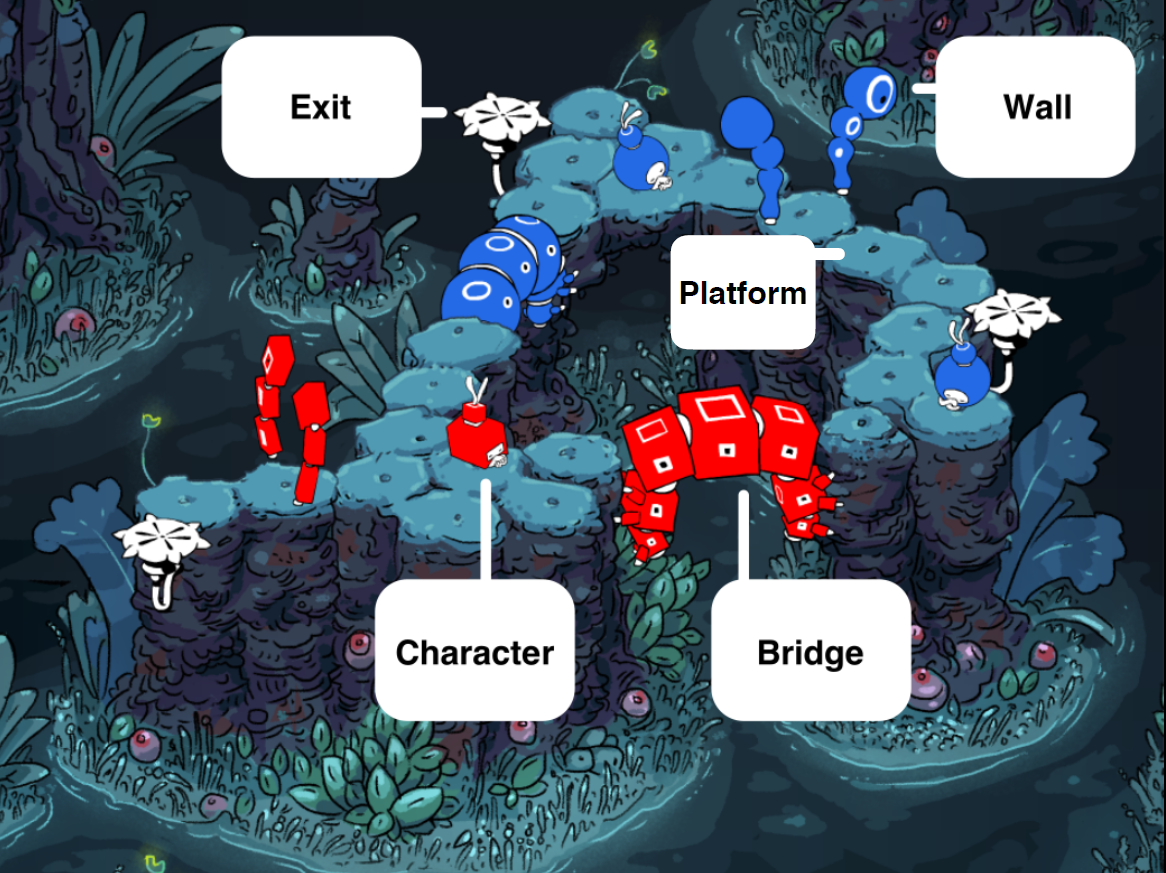
\includegraphics[height=.82\textheight]{../common/figures/she-remembered-caterpillars-game}
		\end{center}
	\end{frame}
	\begin{frame}
		\frametitle{Introduction}
		\framesubtitle{Running Example: She Remembered Caterpillars Ecore Meta-Model}
		\begin{center}
			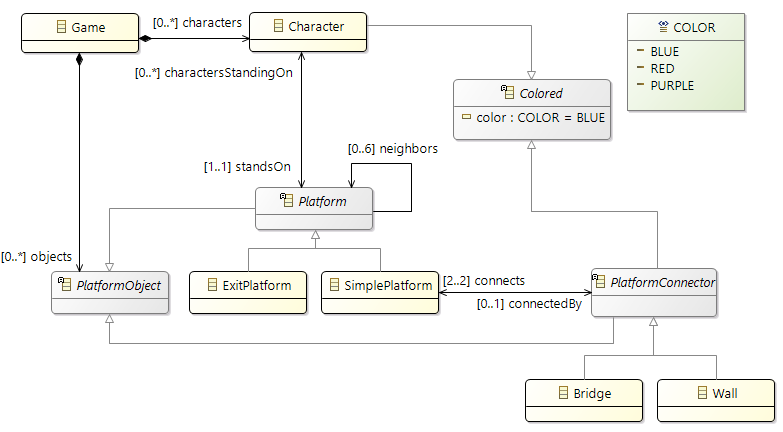
\includegraphics[width=\linewidth]{../common/figures/she-remembered-caterpillars-class-diagram}
		\end{center}
	\end{frame}

\subsection{Unidirectional Graph Transformation}
	\begin{frame}
		\frametitle{Introduction}
		\framesubtitle{Unidirectional Graph Transformation: An Example Rule}
		\begin{center}
			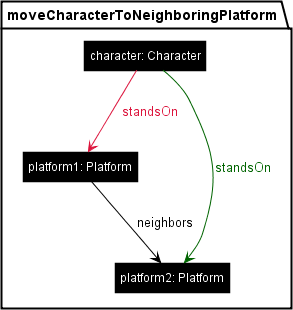
\includegraphics[height=.75\textheight]{../common/figures/rule-moveCharacterToNeighboringPlatform}
		\end{center}
	\end{frame}

\subsection{Main Requirements}
	\begin{frame}
		\frametitle{Introduction}
		\framesubtitle{Main Requirements for a Graph Transformation Tool}
		\begin{enumerate}
			\item Incremental interpreter
				\only<1>{
					\begin{itemize}
						\item Idea: store set of matches of a rule and maintain it whenever the model changes
						\item Pattern matching more efficient 
					\end{itemize}
				}
			\item Integration with a TGG tool
				\only<2>{
					\begin{itemize}
						\item Advantages for developers: shared code, reduce maintenance effort. 
						\item Advantages for users: same meta-models and similar rule syntax for TGGs and GTs
					\end{itemize}
				}
			\item Java API
				\only<3>{
					\begin{itemize}
						\item Easy to use
						\item Type safe
					\end{itemize}
				}
			\item Expressive GT language
				\only<4>{
					\begin{itemize}
						\item Rule refinement
						\item Application conditions
						\item Attribute manipulation
					\end{itemize}
				}
			\item Textual syntax and generated visualization \\
				\only<5>{
					\begin{itemize}
						\item Text for easy editor support and versioning
						\item Visualization for users
					\end{itemize}
				}
		\end{enumerate}
	\end{frame}

\subsection{Comparison of Existing Tools with respect to the Requirements}
	\begin{frame}
		\frametitle{Introduction}
		\framesubtitle{Comparison of Existing Graph Transformation Tools with respect to the Requirements}
		\begin{block}{Comparison Results}
			\begin{itemize}
				\item VIATRA only incremental tool, but no support for GT.
				\item No GT tool supports incrementality.
				\item Most GT tools offer only limited support for application conditions and attribute manipulation.
				\item No GT tool supports rule refinement.
			\end{itemize}
		\end{block}
	\end{frame}
